\chapter{Metodología de la Investigación}
\section{Diseño de la investigación}
En esta parte se describe el diseño de la investigación, el tipo y el enfoque. Asimismo se habla de la población y la muestra.

\subsection{Tipo de investigación}
Se ha identificado que este estudio posee un diseño experimental con el propósito de establecer el tipo de investigación. Según \cite{bk_hernandez2014metodologia} en su obra titulada \citetitle{bk_hernandez2014metodologia}, se pretende determinar el posible efecto de una causa manipulada. Específicamente, se clasifica como un diseño experimental puro debido a la utilización intencionada de variables independientes (modificadas, eliminadas o añadidas) para evaluar su influencia en la variable dependiente, que en este caso es la predicción de las ubicaciones de puntos de acceso (AP) en diversos planos.

\subsection{Enfoque de la investigación}
Este estudio se adhirió a una perspectiva cuantitativa, según lo descrito por \cite{bk_hernandez2014metodologia} en su trabajo \citetitle{bk_hernandez2014metodologia}. Esta perspectiva se centra en la recopilación de datos para verificar hipótesis a través de mediciones numéricas y análisis estadísticos, con el propósito de establecer patrones de comportamiento y validar teorías. Esta metodología se refleja en los diez pasos del proceso cuantitativo mencionados por el autor, los cuales fueron aplicados desde la concepción de la idea hasta la presentación de los resultados finales en el informe de investigación.

\subsection{Población}
Podemos mostrar que la población se compone por los diversos entornos y espacios interiores (planos de edificios, oficinas, centros comerciales, etc.) donde se planea optimizar la cobertura de redes inalámbricas mediante la predicción de ubicaciones para puntos de acceso (APs) utilizando inteligencia artificial generativa.

\subsection{Muestra}
La muestra consistió en 19,154 imágenes de planos interiores en formato vectorial del antecedente \cite{art_wu2019interior}, que se obtuvieron del conjunto RPLAN público. El criterio de selección de esta categoría se basó en los problemas que enfrentan tanto empresas como usuarios en la actualidad con la cobertura Wi-Fi y la ubicación ineficaz de los puntos de acceso interior, lo que resulta en quejas y pérdidas de dinero al realizar una reinstalación o reubicación de estos puntos.

\subsection{Operacionalización de Variables}
Los detalles acerca de cómo se definen y miden las variables de estudio se presentan en la Tabla 1.
%\begin{table}[h!]

\begin{longtable}{>{\raggedright\arraybackslash}m{3cm} >{\raggedright\arraybackslash}m{2cm} >{\raggedright\arraybackslash}m{2cm} >{\raggedright\arraybackslash}m{3cm} >{\raggedright\arraybackslash}m{2cm} >{\raggedright\arraybackslash}m{2.5cm}}
    \caption{Matriz de Variables Principales.}
    \label{tabla:variables}\\
    \hline
    VARIABLE & DIMENSIÓN & INDICADOR & DEFINICIÓN DEL INDICADOR & TÉCNICA DE MEDICIÓN & ESCALA \\
    \hline
    Independiente: Imágenes de Planos Interiores & Calidad de la Imagen & Resolución & Número de píxeles por unidad de área (píxeles por pulgada) & Análisis de propiedades de la imagen & ppi (píxeles por pulgada) \\
    \cline{2-6}
     & Detalle Arquitectónico & Número de Elementos Arquitectónicos Identificables & Cantidad de detalles arquitectónicos (paredes, puertas, ventanas) claramente identificables en la imagen & Contaje manual o mediante software de análisis de imágenes & Número \\
    \hline
    Dependiente: Predicción de Ubicaciones de APs Indoor Con Inteligencia Artificial Generativa & Precisión de la Predicción & Diferencia de Cobertura Predicha vs Real & Diferencia entre la cobertura predicha por el algoritmo y la cobertura real medida & Comparación de resultados de simulación y medición real & Porcentaje \\
    \cline{2-6}
     & Sensibilidad & Tasa de Verdaderos Positivos & Proporción de ubicaciones predichas correctamente como óptimas respecto al total de ubicaciones óptimas reales & Evaluación de predicciones respecto a un conjunto de prueba & Porcentaje \\
    \cline{2-6}
     & Puntaje F1 & Media Armónica de Precisión y Sensibilidad & Combina la precisión y la sensibilidad en un solo valor & Evaluación de predicciones respecto a un conjunto de prueba & Valor F1 \\
    \cline{2-6}
     & Área Bajo la Curva ROC & AUC-ROC & Medida de la capacidad del modelo para distinguir entre clases & Evaluación de la curva ROC & Valor AUC \\
    \hline
\end{longtable}
%\par	%%Salto de linea
%\bigskip
\begin{flushleft}	%%Alinear a la izquierda sin justificar
	\small Fuente: Elaboración propia.
\end{flushleft}
%\end{table}

\section{Técnicas de recolección de datos}
La recolección de planos interiores es un paso crucial para la optimización de la cobertura de redes inalámbricas mediante la inteligencia artificial generativa. Una de las técnicas más accesibles y efectivas para obtener estos planos es a través del uso de bases de datos públicas y repositorios en línea. Estas fuentes ofrecen una amplia variedad de planos de planta, que pueden ser utilizados para modelar y predecir las ubicaciones óptimas de puntos de acceso (APs) en diferentes entornos interiores.

\begin{figure}[h]
	\begin{center}
		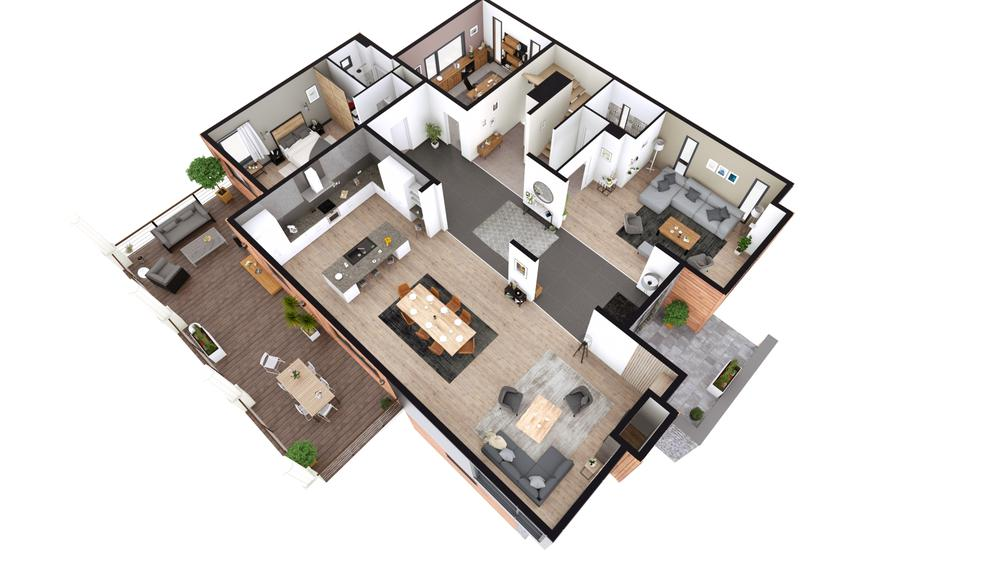
\includegraphics[width=0.75\textwidth]{3/figures/plano2d.jpg}
		\caption[Plano interior]{Plano interior.\\
			Fuente: \cite{art_wu2019interior}.}
		\label{3:fig1}
	\end{center}
\end{figure}

\begin{itemize}
    \item \textbf{Repositorios de Arquitectura y Diseño}: Existen múltiples repositorios en línea dedicados específicamente a la arquitectura y el diseño. Sitios web como ArchDaily, Floorplanner y otros, ofrecen planos de planta y modelos 3D de edificios que pueden ser descargados y utilizados para diversos fines. Estos repositorios suelen incluir planos de diferentes tipos de edificios, desde residenciales hasta comerciales y educativos, lo que proporciona una amplia gama de opciones para la optimización de redes inalámbricas.
    \item \textbf{Bibliotecas Digitales y Bases de Datos Académicas}: Las bibliotecas digitales y bases de datos académicas son otra fuente valiosa para la recolección de planos interiores. Instituciones académicas y bibliotecas públicas a menudo mantienen colecciones de planos de edificios históricos y contemporáneos. Plataformas como JSTOR, Google Scholar y las bibliotecas digitales universitarias pueden contener planos de planta detallados en publicaciones académicas, tesis y proyectos de investigación.
    \item \textbf{Plataformas de Colaboración y Repositorios de Código Abierto}: Plataformas como GitHub y otros repositorios de código abierto también pueden ser recursos útiles para la recolección de planos interiores. Investigadores y profesionales de la industria a menudo comparten conjuntos de datos, modelos y planos como parte de sus proyectos de colaboración. Estos recursos pueden ser utilizados libremente bajo licencias abiertas, lo que facilita su integración en proyectos de optimización de redes inalámbricas.
    \item \textbf{Repositorios de Proyectos de Construcción}: Sitios web como Procore y otros repositorios de gestión de proyectos de construcción ofrecen planos y documentos relacionados con proyectos de construcción. Estos repositorios son utilizados por profesionales de la construcción para gestionar y compartir información sobre proyectos, y a menudo incluyen planos de planta detallados que pueden ser utilizados para análisis posteriores.
    \end{itemize}



%\newpage
\section{Técnicas para el procesamiento y análisis de la información}

\subsection{Metodología de implementación de la solución}

La producción de imágenes mediante Inteligencia Artificial Generativa involucra varias fases de desarrollo, que van desde la recopilación de imágenes hasta su interpretación, como se menciona en el trabajo de \cite{tec_kingma2019variat}. La imagen adquirida debe pasar por un proceso detallado posteriormente para alcanzar su etapa final. La metodología del presente trabajo de investigación se ilustra en la Figura 37.

\begin{figure}[h]
	\begin{center}
		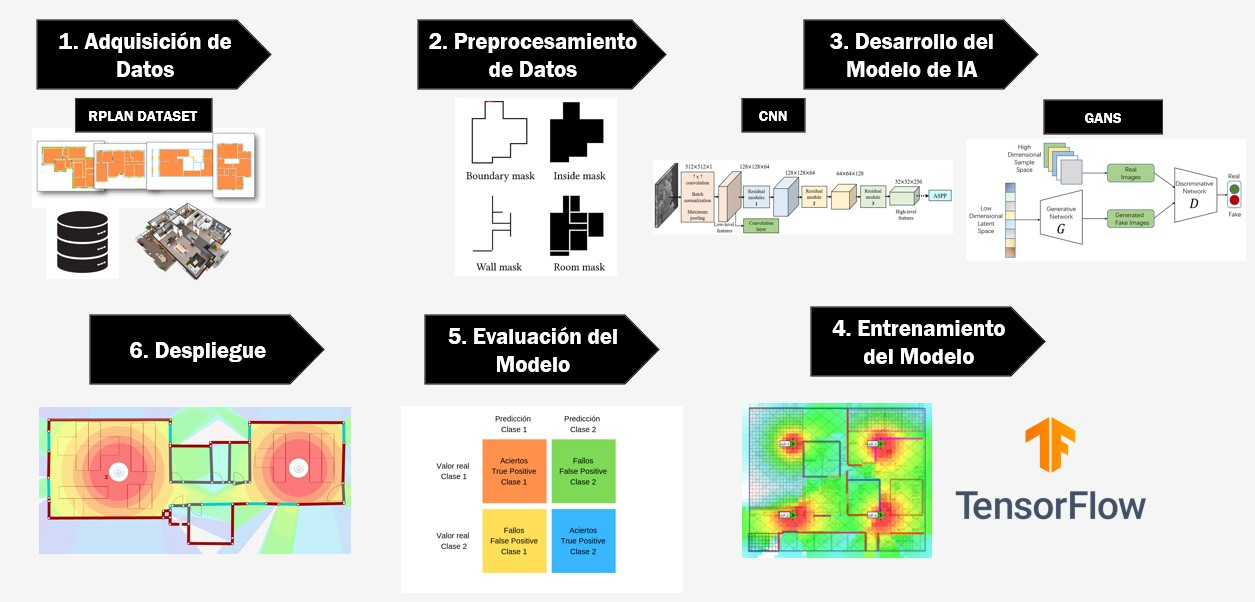
\includegraphics[width=1.1\textwidth]{3/figures/metodologia.jpg}
		\caption[Metodología de la Investigación]{Metodología de la Investigación.\\
			Fuente: Elaboración propia.}
		\label{3:fig2}
	\end{center}
\end{figure}

\newpage
\subsubsection{Adquisición de Datos}

En esta sección se detalla el procedimiento empleado para obtener el conjunto de datos utilizado en este estudio. A continuación se presenta una tabla que resume las tareas y actividades llevadas a cabo durante esta fase de adquisición. El primer paso consistió en recopilar los datos. Los detalles sobre las actividades y tareas se encuentran en la Tabla 2.

\begin{longtable}{>{\raggedright\arraybackslash}p{4cm} >{\raggedright\arraybackslash}p{4cm} >{\raggedright\arraybackslash}p{5cm}}
    \caption{Tabla de la Adquisición de Datos.}
    \label{tabla:actividades}\\
    \hline
    \textbf{Actividades} & \textbf{Descripción} & \textbf{Tareas}\\
    \hline
    \endfirsthead

    \multicolumn{3}{c}%
    {{\bfseries \tablename\ \thetable{} -- continuación de la página anterior}} \\
    \hline
    \textbf{Actividades} & \textbf{Descripción} & \textbf{Tareas}\\
    \hline
    \endhead

    \hline
    \multicolumn{3}{r}{{Continúa en la siguiente página}} \\
    \endfoot

    \hline
    \endlastfoot

    Localización de bases de datos que contengan imágenes de planos interiores de planta con dimensiones idénticas y características similares. & Localización de bases de datos que contengan imágenes de planos interiores de planta pertinentes para la investigación. & 
    \begin{itemize}
        \item Analizar y identificar bases de datos con planos de planta interiores.
        \item Confirmar que la base de datos esté disponible públicamente y sea pertinente para el estudio.
        \item Descargar los datos desde el repositorio apropiado.
    \end{itemize} \\
\end{longtable}


\begin{flushleft}
    \small Fuente: Elaboración propia.
\end{flushleft}

A continuación, se proporciona un detalle de cada actividad mencionada en la tabla anterior, junto con los resultados que se esperan obtener.

\textbf{Actividad 1: Localización de bases de datos que contengan imágenes de planos interiores de planta con dimensiones idénticas y características similares}
\\
Esta actividad explica la identificación de la base de datos. Para la base de datos, se obtuvieron más de ochenta mil planos de plantas de edificios residenciales reales de la base de datos pública RPLAN, que recolectó planos del mercado inmobiliario de Asia en 2019. Las imágenes de planos interiores se encuentran en la base de datos. La Figura 38 muestra ejemplos de cómo es la data. Cada plano de planta tiene gráficos vectoriales dentro de una región cuadrada de 18m × 18m con elementos geométricos e información semántica, y cada plano de planta tiene una imagen de 256 × 256.


\textbf{Entregable}: Dataset, creado en Asia, contiene imágenes de planos interiores del mercado inmobiliario asiático.


\subsubsection{Preprocesamiento de Datos}
Se realizará el preprocesamiento de las imágenes del conjunto en esta etapa. La tabla 3 incluye las tareas y actividades necesarias para completar la etapa de preprocesamiento:
\vspace{2ex}


\begin{longtable}{|p{3cm}|p{3cm}|p{9cm}|}
    \caption{Actividades de la fase de Preprocesamiento de Datos.}
    \label{tabla:preprocesamiento}\\
    \hline
    \textbf{Actividades} & \textbf{Descripción} & \textbf{Tareas} \\
    \hline
    \endfirsthead

    \hline
    \textbf{Actividades} & \textbf{Descripción} & \textbf{Tareas} \\
    \hline
    \endhead

    \hline
    \endfoot

    \hline
    \endlastfoot

    Filtración de las imágenes de los planos interiores& Filtrado de datos no estándar para evitar interferencias y mejorar la fiabilidad del conjunto de datos. & 
    \begin{itemize}
        \item Eliminar planos de planta que contengan tipos de habitaciones indefinidas o de muy baja frecuencia.
        \item Mantener planos de planta que cumplan con los siguientes requisitos:
        \begin{enumerate}
            \item Área total del plano de planta superior a 60 m² y menor a 120 m².
            \item Número de habitaciones en el plano de planta mayor que 3 y menor que 9.
            \item El plano de planta tiene sala de estar.
            \item La proporción del área de la sala de estar respecto al área total del plano de planta es mayor que 0.25 y menor que 0.55.
            \item El área promedio de cada habitación es mayor a 10 m² y menor a 20 m².
        \end{enumerate}
    \end{itemize} \\
    \hline
    Representación de las imágenes de los planos interiores& Representación de cada plano de planta como una imagen de cuatro canales. & 
    \begin{itemize}
        \item Guardar la máscara interior en el primer canal.
        \item Almacenar la información de límites en el segundo canal.
        \item Representar la semántica de habitaciones y paredes en el tercer canal con números enteros específicos.
        \item Usar el cuarto canal para almacenar información adicional que distinga entre diferentes habitaciones con las mismas etiquetas. Diferentes números enteros se utilizan para distinguir habitaciones con las mismas etiquetas.
    \end{itemize} \\
    \hline
    \caption{Actividades de la fase de Preprocesamiento de Datos.}
    \label{tabla:actividades}
\end{longtable}


%\par	%%Salto de linea
%\bigskip
\begin{flushleft}	%%Alinear a la izquierda sin justificar
	\small Fuente: Elaboración propia.
\end{flushleft}

A continuación, se describe en detalle cada actividad junto con el resultado esperado.

\textbf{Actividad 1: Filtración de las imágenes de los planos interiores}
\\
En la fase de preprocesamiento de datos, la actividad de Filtración se enfoca en depurar y mejorar la calidad del conjunto de datos al eliminar información irrelevante o poco confiable. Esto se logra a través de la eliminación de datos no estándar y la conservación de aquellos que cumplen con criterios específicos de relevancia y fiabilidad. 

\textbf{Entregable}: Conjunto de datos filtrado y optimizado para su posterior análisis.

\textbf{Actividad 2: Representación de las imágenes de los planos interiores}
\\
Por otro lado, la actividad de Representación se encarga de convertir los datos en un formato visual o estructurado más adecuado para su análisis y comprensión. Esto implica transformar los datos en imágenes o representaciones gráficas que faciliten su visualización y entendimiento, contribuyendo así a una mejor interpretación por parte de los usuarios finales, como podemos observar en la Figura 38.

\textbf{Entregable}: Representación visual y estructurada de cada plano de planta en un formato adecuado para su procesamiento y análisis posterior.

\begin{figure}[h]
    \begin{center}
        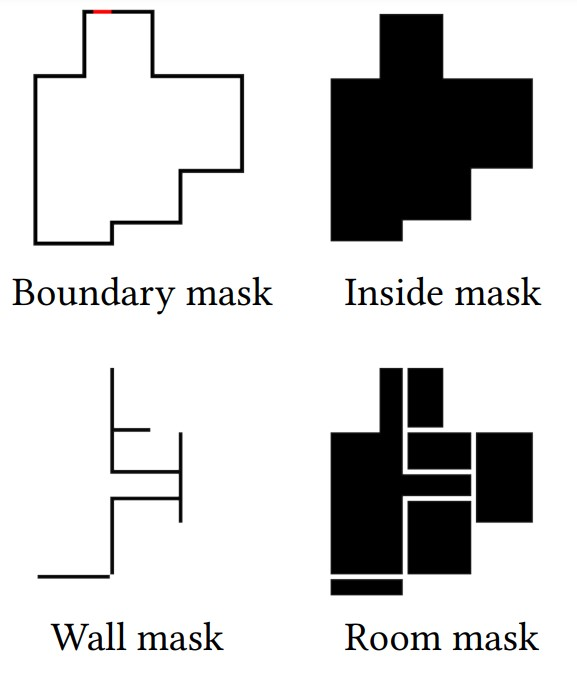
\includegraphics[width=0.5\textwidth]{3/figures/Representacion_planos.jpg}
        \caption[Representación de las imágenes de los planos interiores]{Representación de las imágenes de los planos interiores.\\
        Fuente: \cite{art_wu2019interior}. \citetitle{art_wu2019interior}.}
        \label{3:fig3}
    \end{center}
\end{figure}

\subsubsection{Desarrollo del Modelo de IA}
Tres actividades fundamentales componen el modelo generativo para la optimización de la cobertura de las redes inalámbricas para la predicción de las ubicaciones de los puntos de acceso. Cada una de estas actividades utiliza estrategias de aprendizaje profundo avanzadas para trabajar de manera secuencial y colaborativa. La Tabla 4 muestra todo esto más a fondo.

\vspace{2ex}
\begingroup
\renewcommand\arraystretch{0.3}
\begin{longtable}{|p{4cm}|p{6cm}|p{6cm}|}
    \caption{Actividades de la fase de Desarrollo del Modelo de IA.}
    \label{tabla:actividades}\\
    \hline
    \textbf{Actividades} & \textbf{Descripción} & \textbf{Tareas} \\
    \hline
    \endfirsthead
    
    \multicolumn{3}{c}%
    {{\bfseries \tablename\ \thetable{} -- continuación de la página anterior}} \\
    \hline
    \textbf{Actividades} & \textbf{Descripción} & \textbf{Tareas} \\
    \hline
    \endhead
    
    \hline \multicolumn{3}{|r|}{{Continúa en la próxima página}} \\
    \hline
    \endfoot
    
    \hline
    \endlastfoot
    
    Arquitectura de la Red & Diseñar la arquitectura de la red neuronal para la predicción de APs. & 
    \begin{itemize}
        \item Selección del tipo de red CNN y GAN.
        \item Diseño de la arquitectura de la red (capas convolucionales).
        \item Implementación de la red en un framework de aprendizaje profundo.
        \item Definición de entradas y salidas.
    \end{itemize} \\
    \hline
    
    \end{longtable}
\endgroup

%\par	%%Salto de linea
%\bigskip
\begin{flushleft}	%%Alinear a la izquierda sin justificar
	\small Fuente: Elaboración propia
\end{flushleft}

A continuación, se proporciona un detalle de cada actividad junto con el entregable correspondiente que se espera obtener.

\textbf{Actividad 1: Arquitectura de la Red}
\\
Durante esta etapa, se llevará a cabo el diseño e implementación de la arquitectura de una red neuronal destinada a predecir las ubicaciones de puntos de acceso (APs). Se empleará una combinación de Redes Neuronales Convolucionales (CNN) y Redes Generativas Antagónicas (GANs) para aprovechar sus capacidades en la extracción de características espaciales y la generación de soluciones óptimas.

Respecto, al proceso de Red Neuronal Convolucional (CNN) para la extracción de características, podemos verla con más detalle en la Figura 39, donde se ve el uso de la capa Conv2D (Varias capas convolucionales para extraer características espaciales), la capa MaxPooling2D (Capas de pooling para reducir dimensionalidad y mantener características importantes), la capa Flatten (Aplanar la salida para conectarla con capas densas) y finalmente la capa Dense (Capas densas para aprendizaje y combinación de características extraídas).

\begin{figure}[H]
	\centering
	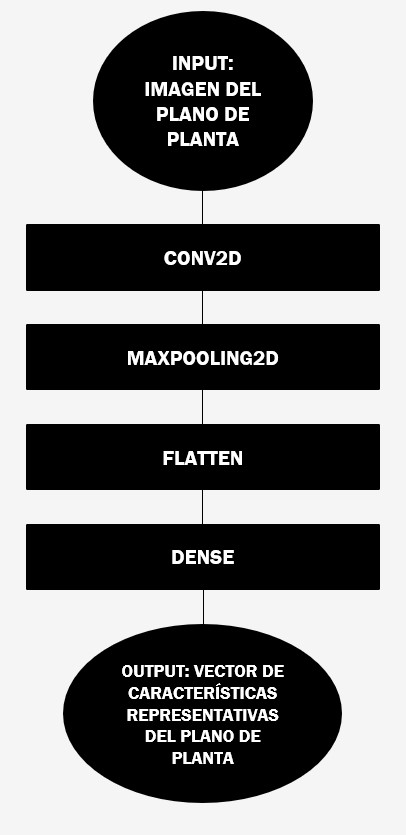
\includegraphics[width=0.3\textwidth]{3/figures/CNN_redneuro.jpg}
	\caption[CNN para el análisis y extracción de rasgos característicos]{CNN para el análisis y extracción de rasgos característicos.\\ Fuente: Elaboración propia.}
	\label{3:4}
\end{figure}


Por consiguiente, al proceso del Generador del GAN, podemos verla con más detalle en la Figura 40, donde se ve el uso de la capa Dense (Varias capas densas para transformar el vector de características en un plano con las ubicaciones de los Aps), la capa Reshape (Dar forma al plano para que corresponda con las dimensiones del plano de planta), la capa Flatten (Aplanar la salida para conectarla con capas densas) y finalmente la capa Conv2DTranspose (Capas convolucionales transpuestas para generar la imagen final).

\begin{figure}[H]
	\centering
	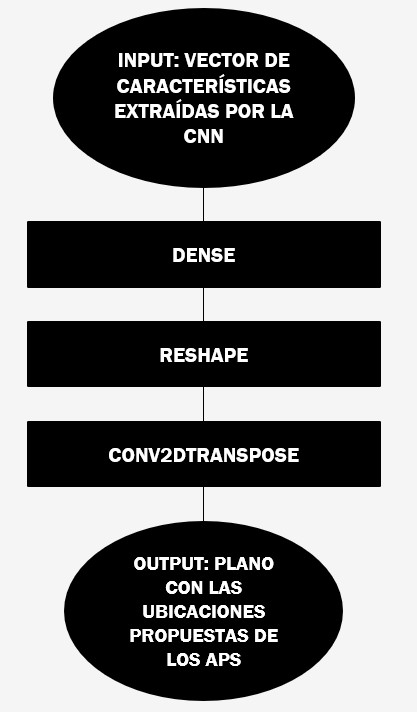
\includegraphics[width=0.4\textwidth]{3/figures/gans_capas.jpg}
	\caption[Generador del GAN]{Generador del GAN.\\ Fuente: Elaboración propia.}
	\label{3:5}
\end{figure}

Finalmente, al proceso del Discriminador del GAN, podemos verla con más detalle en la Figura 41, donde se ve el uso de la capa Conv2D (Varias capas convolucionales para analizar la imagen y evaluar la calidad de las ubicaciones propuestas), la capa MaxPooling2D (Capas de pooling para reducir dimensionalidad), la capa Flatten (Aplanar la salida para conectarla con capas densas) y finalmente la capa Dense (Capas densas para la clasificación final).

\begin{figure}[H]
	\centering
	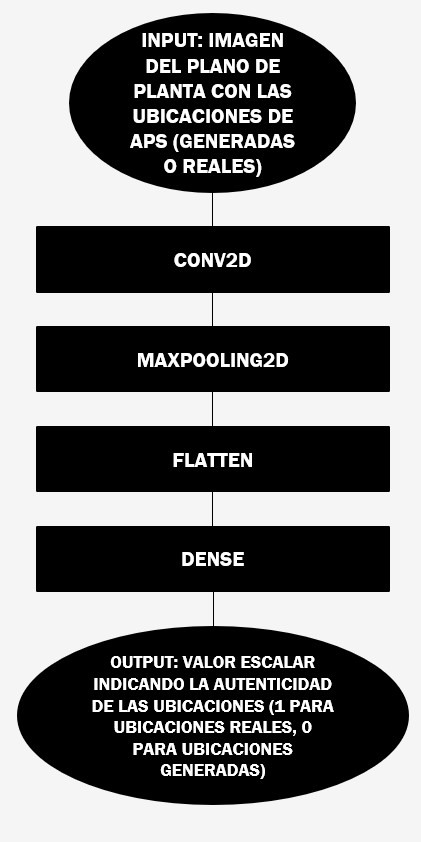
\includegraphics[width=0.4\textwidth]{3/figures/discrimGAN.jpg}
	\caption[Discriminador del GAN]{Discriminador del GAN.\\ Fuente: Elaboración propia.}
	\label{3:6}
\end{figure}

A todo ello se se utilizará TensorFlow para implementar la arquitectura descrita. A continuación, se presenta un pseudocódigo para la implementación en la Figura 42.

\begin{figure}[H]
	\centering
	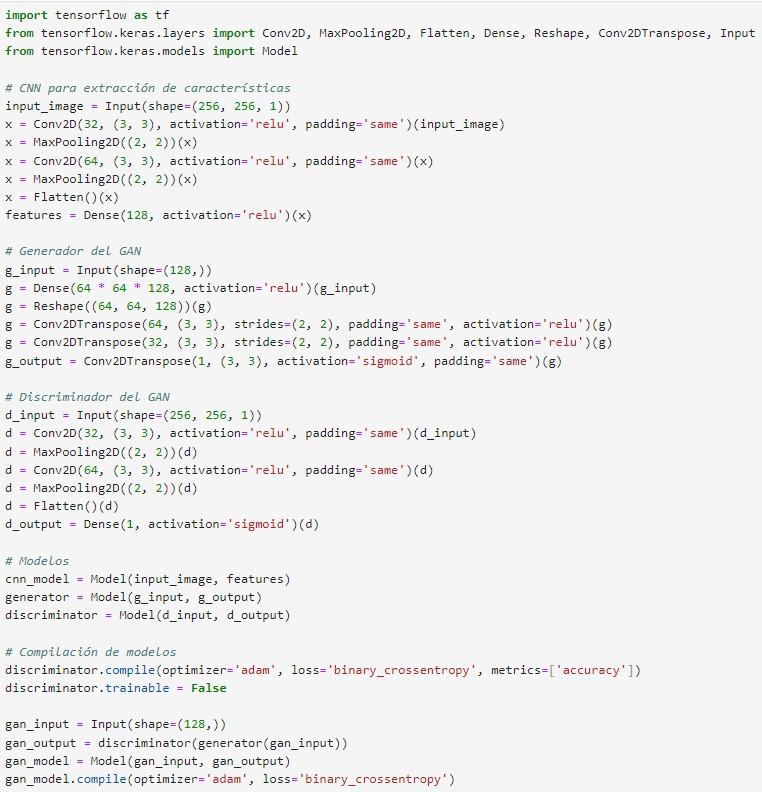
\includegraphics[width=1\textwidth]{3/figures/pseudocodigo.jpg}
	\caption[Pseudocódigo para la implementación]{Pseudocódigo para la implementación.\\ Fuente: Elaboración propia.}
	\label{3:7}
\end{figure}

\textbf{Entregable}: Código fuente de la red neuronal implementada, Diagramas y especificaciones de la arquitectura de la red y Especificaciones de entrada y salida del modelo.

\subsubsection{Entrenamiento del Modelo}
Al concluir la etapa del Desarrollo del Modelo de IA, se continua con el Entrenamiento, en la Tabla 5 fueron diseñados siguiendo las actividades.

\vspace{2ex}
\begingroup
\renewcommand\arraystretch{0.3}
\begin{longtable}{|p{4cm}|p{6cm}|p{6cm}|}
    \caption{Actividades del Entrenamiento del Modelo.}
    \label{tabla:actividades}\\
    \hline
    \textbf{Actividades} & \textbf{Descripción} & \textbf{Tareas} \\
    \hline
    \endfirsthead
    
    \multicolumn{3}{c}%
    {{\bfseries \tablename\ \thetable{} -- continuación de la página anterior}} \\
    \hline
    \textbf{Actividades} & \textbf{Descripción} & \textbf{Tareas} \\
    \hline
    \endhead
    
    \hline \multicolumn{3}{|r|}{{Continúa en la próxima página}} \\
    \hline
    \endfoot
    
    \hline
    \endlastfoot
    
    Entrenamiento Supervisado & Utilizar datos anotados para entrenar el modelo de predicción de APs. & 
    \begin{itemize}
        \item Entrenamiento del modelo utilizando el dataset anotado.
        \item Evaluación y ajuste de hiperparámetros.
    \end{itemize} \\
    \hline
    
    Optimización de Cobertura & Entrenar el modelo para maximizar la cobertura y minimizar la interferencia. & 
    \begin{itemize}
        \item Uso de técnicas de regularización para evitar sobreajuste.
        \item Simulaciones para evaluar el impacto de las predicciones de APs en la cobertura de red.
        \item Ajuste iterativo del modelo basado en los resultados de las simulaciones.
    \end{itemize} \\
    \hline
    
    \end{longtable}
\endgroup

\textbf{Actividad 1: Entrenamiento Supervisado}
\\
El entrenamiento supervisado implica el uso de un conjunto de datos anotado donde las ubicaciones óptimas de los puntos de acceso (APs) están previamente definidas. Este proceso es fundamental para enseñar al modelo a reconocer patrones y aprender a predecir ubicaciones óptimas de APs en base a la disposición de los planos de planta.
Asimismo, se elaboró el pseudocódigo el cual se puede ver en la Figura 43.

\begin{figure}[H]
	\centering
	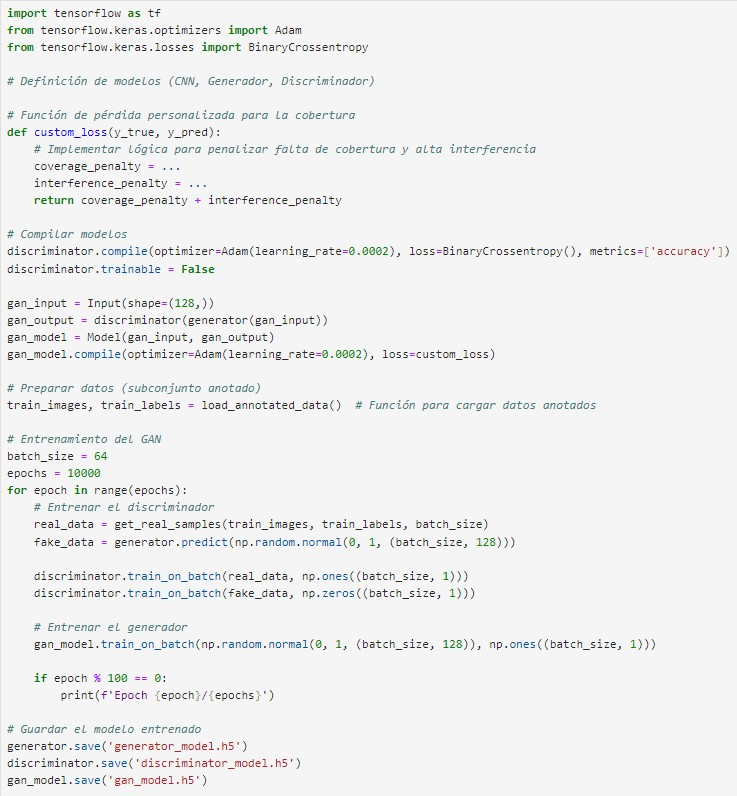
\includegraphics[width=1\textwidth]{3/figures/pseudo_train.jpg}
	\caption[Pseudocódigo para el Entrenamiento Supervisado]{Pseudocódigo para el Entrenamiento Supervisado.\\ Fuente: Elaboración propia.}
	\label{3:8}
\end{figure}

\textbf{Entregable}: Modelo entrenado y archivos de checkpoints.

\textbf{Actividad 2: Optimización de Cobertura}
\\
La optimización de la cobertura implica ajustar el modelo para maximizar la cobertura de red y minimizar la interferencia. Esto se logra implementando métricas específicas en la función de pérdida y realizando simulaciones de cobertura.

Asimismo, se elaboró el pseudocódigo el cual se puede ver en la Figura 44.

\begin{figure}[H]
	\centering
	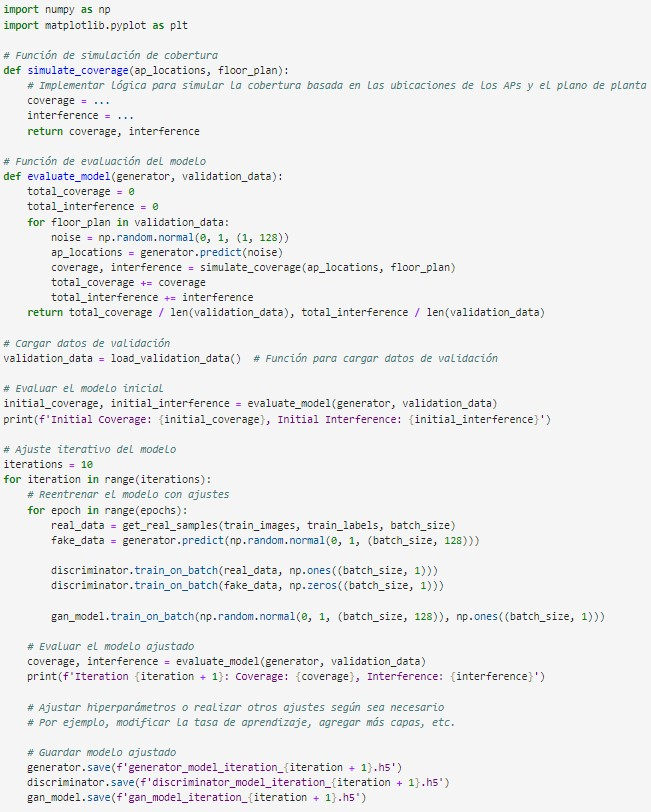
\includegraphics[width=1\textwidth]{3/figures/pseudo_cobert.jpg}
	\caption[Pseudocódigo para la Optimización de Cobertura]{Pseudocódigo para la Optimización de Cobertura.\\ Fuente: Elaboración propia.}
	\label{3:9}
\end{figure}

\textbf{Entregable}: Función de pérdida mejorada con métricas de cobertura e interferencia y Reporte de resultados de simulaciones de cobertura.

\subsubsection{Evaluación del Modelo}
Durante esta fase, se lleva a cabo la evaluación de los modelos creados en la investigación utilizando las métricas de clasificación seleccionadas y explicadas en la sección 3.3.2. En la Tabla 6 se detallan las actividades y tareas realizadas en esta etapa.

%\vspace{2ex}
%\begingroup
%\renewcommand\arraystretch{0.3}
\begin{longtable}{|>{\raggedright\arraybackslash}p{4cm}|>{\raggedright\arraybackslash}p{5cm}|>{\raggedright\arraybackslash}p{6cm}|}
    \caption{Actividades de la Evaluación del Modelo.}
    \label{tabla:actividades}\\
    \hline
    \textbf{Actividad} & \textbf{Descripción} & \textbf{Tareas} \\
    \hline
    \endfirsthead

    \hline
    \textbf{Actividad} & \textbf{Descripción} & \textbf{Tareas} \\
    \hline
    \endhead

    \hline
    \endfoot

    \hline
    \endlastfoot

    Preparación de Datos de Validación & Seleccionar y preparar un conjunto de datos de validación representativo. & 
    \begin{itemize}
        \item Elección de planos de planta que no hayan sido empleados en el proceso de entrenamiento.
        \item Preprocesamiento de imágenes.
    \end{itemize} \\
    \hline
    Definición de Métricas de Evaluación & Definir métricas cuantitativas para evaluar la cobertura y la interferencia. & 
    \begin{itemize}
        \item Identificación de métricas adecuadas.
        \item Implementación de funciones para calcular estas métricas.
    \end{itemize} \\
    \hline
    Evaluación del Modelo & Evaluar el modelo entrenado en el conjunto de datos de validación para obtener una línea base. & 
    \begin{itemize}
        \item Predicción de ubicaciones de APs en el conjunto de validación.
        \item Cálculo de métricas de evaluación.
    \end{itemize} \\
    \hline
\end{longtable}
%\endgroup
%\par	%%Salto de linea
%\bigskip
\begin{flushleft}	%%Alinear a la izquierda sin justificar
	\small Fuente: Elaboración propia
\end{flushleft}

\textbf{Actividad 1: Preparación de Datos de Validación}
\\
La preparación de los datos de validación desempeña un papel crucial en la evaluación de la efectividad del modelo en datos no previamente vistos. Esta tarea implica seleccionar un subconjunto representativo del conjunto de datos que no se haya utilizado durante el entrenamiento del modelo. La selección debe tener en cuenta la diversidad en los planos de planta y sus configuraciones para garantizar que el modelo pueda generalizar correctamente a diferentes escenarios.

\textbf{Entregable}: Un conjunto de datos listo para su uso en la evaluación del modelo, que incluye imágenes preprocesadas y listas para ser utilizadas en el análisis.

\textbf{Actividad 2: Definición de Métricas de Evaluación}
\\
Para evaluar el rendimiento del modelo de manera cuantitativa, es esencial definir métricas claras que reflejen tanto la cobertura de la red como los niveles de interferencia. Estas métricas proporcionarán una base objetiva para comparar el rendimiento del modelo en diferentes escenarios y con otros enfoques existentes.

\textbf{Entregable}: Un documento detallado que describe cada métrica y proporciona el código o las funciones necesarias para calcularlas.

\vspace{0.5cm}
\textbf{Actividad 3: Evaluación del Modelo}
\\
La evaluación del modelo involucra el uso del conjunto de datos de validación para establecer un punto de referencia sobre su rendimiento. Esta evaluación es esencial para comprender el comportamiento del modelo en situaciones no previamente vistas durante el entrenamiento y para identificar posibles áreas de mejora.

\textbf{Entregable}: Un informe que presenta los resultados de la evaluación inicial, incluyendo las métricas de rendimiento calculadas y cualquier observación relevante sobre el comportamiento del modelo.

\subsubsection{Despliegue}
En la etapa final de la metodología empleada, se procedió a implementar el modelo propuesto una vez finalizados su entrenamiento y evaluación respectiva. Las actividades realizadas en esta fase se detallan en la Tabla 7.

%\vspace{2ex}
%\begingroup
%\renewcommand\arraystretch{0.3}
\begin{longtable}{|>{\raggedright\arraybackslash}p{4cm}|>{\raggedright\arraybackslash}p{5cm}|>{\raggedright\arraybackslash}p{6cm}|}
    \caption{Actividades del Despliegue.}
    \label{tabla:actividades}\\
    \hline
    \textbf{Actividad} & \textbf{Descripción} & \textbf{Tareas} \\
    \hline
    \endfirsthead

    \hline
    \textbf{Actividad} & \textbf{Descripción} & \textbf{Tareas} \\
    \hline
    \endhead

    \hline
    \endfoot

    \hline
    \endlastfoot

    Preparación del Entorno de Despliegue & Configurar el entorno necesario para desplegar el modelo en producción. & 
    \begin{itemize}
        \item Selección de infraestructura.
        \item Configuración del entorno de hardware y software.
        \item Pruebas iniciales.
    \end{itemize} \\
    \hline
    Despliegue del Modelo en Producción & Implementar el modelo en el entorno de producción para su uso real. & 
    \begin{itemize}
        \item Implementación del modelo en producción.
        \item Configuración de parámetros en tiempo de ejecución.
        \item Monitoreo inicial del desempeño.
    \end{itemize} \\
    \hline
\end{longtable}
%\endgroup
%\par	%%Salto de linea
%\bigskip
\begin{flushleft}	%%Alinear a la izquierda sin justificar
	\small Fuente: Elaboración propia
\end{flushleft}

\textbf{Actividad 1: Preparación del Entorno de Despliegue}
\\
La preparación del entorno de despliegue es una etapa fundamental para asegurar que el modelo de IA pueda ser ejecutado eficientemente en producción. Este proceso implica la selección y configuración de la infraestructura necesaria, incluyendo tanto hardware como software, y la realización de pruebas iniciales para confirmar que todo funciona correctamente antes del despliegue completo.

\textbf{Entregable}: Un entorno completamente preparado, con todos los componentes necesarios instalados y configurados, listo para el despliegue del modelo.

\vspace{0.25cm}
\textbf{Actividad 2: Despliegue del Modelo en Producción}
\\
El despliegue del modelo en producción es el paso en el que el modelo de IA se pone en funcionamiento en el entorno de producción. Este proceso incluye la implementación del modelo, la configuración de parámetros necesarios para su ejecución en tiempo real, y el monitoreo inicial para asegurar que el modelo funciona correctamente en condiciones reales.

\textbf{Entregable}: El modelo está completamente implementado y operando en el entorno de producción, con los parámetros ajustados y el desempeño monitoreado para asegurar su correcto funcionamiento.

\vspace{0.5cm}
\subsection{Metodología para la medición de resultados}
Diversas métricas se emplean para evaluar el desempeño de un modelo, sirviendo como herramientas de evaluación fundamentadas en los datos de la Matriz de Confusión. A continuación, se detalla su concepto y sus componentes.

\begin{itemize}
\item \textbf{Matriz de confusión}: La Matriz de Confusión es una tabla de dimensiones NxN que sintetiza la precisión de las predicciones generadas por un modelo de clasificación. Esta matriz muestra la relación entre las etiquetas predichas por el modelo y las etiquetas reales de los datos. Uno de los ejes de la matriz representa las etiquetas predichas, mientras que el otro muestra las etiquetas reales, con N representando el número total de clases. En el contexto de un problema de clasificación binaria, N=2 \parencite{gl_kohavi1998ml_glossary}. Su objetivo principal es evaluar el rendimiento de un modelo de Machine Learning supervisado en datos de prueba, donde las etiquetas reales son desconocidas. El término "matriz de confusión" se origina porque ayuda a identificar dónde el sistema confunde entre dos clases (Big Data, 2019). Puedes encontrar una representación visual de la matriz de confusión en la Figura 45.
\begin{figure}[H]
	\centering
	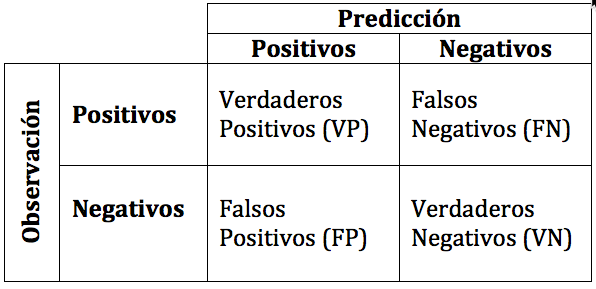
\includegraphics[width=0.75\textwidth]{3/figures/matriz_confusion.png}
	\caption[Matriz de Confusión]{Matriz de Confusión.\\ Fuente: \cite{gl_izco2018bdc}. \citetitle{gl_izco2018bdc}.}
	\label{3:9}
\end{figure}
\end{itemize}

\begin{itemize}
    \item \textbf{Verdaderos Positivos}: Se denomina verdadero positivo cuando el modelo realiza una predicción precisa de la clase positiva.
    \item \textbf{Verdaderos Negativos}: Se trata de un verdadero negativo cuando el modelo realiza una predicción correcta de la clase negativa.
    \item \textbf{Falsos Positivos}: Ocurre un falso positivo cuando el modelo hace una predicción incorrecta de la clase positiva. 
    \item \textbf{Falsos Negativos}: Ocurre un falso negativo cuando el modelo hace una predicción incorrecta de la clase negativa. 
    \end{itemize}

    Después de explicar los conceptos previos, se obtienen las siguientes métricas comúnmente utilizadas en clasificación, de las cuales se utilizarán solo las tres primeras según lo referenciado en los documentos anteriores:

    \begin{itemize}
    \item \textbf{Exactitud}: es una medida que representa la proporción de predicciones correctas sobre el total de ejemplos en un modelo de clasificación. Se calcula utilizando la siguiente fórmula \parencite{gl_kohavi1998ml_glossary}:
	%\begin{equcaption}[!ht]
    \begin{equation}\label{eq:accuracy}
        \phantomsection
        Exactitud=\frac{V.P.+V.N.}{V.P.+V.N.+F.P.+F.N.}
        \end{equation}
        \myequations{Fórmula para la exactitud}
        
        La pregunta que responde esta métrica es ¿Cuál es la proporción de predicciones correctas? 
        
        \item \textbf{Precisión}: mide el número de elementos correctamente identificados como positivos en relación al total de elementos identificados como positivos. Se calcula utilizando la siguiente fórmula:
        \begin{equation}\label{eq:precision}
        \phantomsection
        Precisi\acute{o}n=\frac{V.P.}{V.P.+F.P.}
        \end{equation}
        \myequations{Fórmula para la precisión}
        
        La pregunta que responde esta métrica es: ¿Cuál es la proporción de predicciones positivas que son precisas?

	\item \textbf{Área bajo la curva ROC}: Esta métrica considera todos los umbrales de clasificación posibles y representa la probabilidad de que un clasificador esté más seguro de que un ejemplo sea un verdadero positivo en lugar de un falso positivo \parencite{gl_google2018machinelearning}. Para comprender esta métrica, es necesario entender primero qué es la curva ROC y su utilidad.
	
    La curva ROC es una herramienta que evalúa la capacidad de distinguir entre dos categorías en un modelo, como por ejemplo, determinar si un paciente tiene cáncer o no.

Al ajustar el umbral hacia la izquierda, lo que aumenta la sensibilidad, la especificidad tiende a disminuir. Por otro lado, al mover el umbral hacia la derecha, disminuye la sensibilidad y aumenta la especificidad. El AUC representa la sensibilidad (1-especificidad) \parencite{gl_gonzalez2019auc}.

El área bajo esta curva indica qué tan efectivo es el modelo. Un mayor rendimiento se refleja en una curva que se aleja de la diagonal principal, como se calcula con la siguiente fórmula:

\begin{equation}\label{eq
}
\phantomsection
P(\text{score}(x^{+}) > \text{score}(x^{-}))
\end{equation}
\myequations{Fórmula para el área bajo la curva ROC}
En cuanto a la interpretación del área bajo la curva ROC, se establece lo siguiente:
\begin{itemize}
    \item Si el valor es igual a 0.5, indica que el modelo no tiene capacidad discriminativa.
    \item Si el valor está entre 0.5 y 0.7, se considera que la capacidad discriminativa del modelo es insatisfactoria.
    \item Si el valor está entre 0.7 y 0.8, se considera que la capacidad discriminativa del modelo es aceptable.
    \item Si el valor está entre 0.8 y 0.9, se considera que la capacidad discriminativa del modelo es excelente.
    \item Si el valor es igual o mayor a 0.9, se considera que la capacidad discriminativa del modelo es excepcionalmente buena.
    \end{itemize}
	\item \textbf{Sensibilidad}: Mide la proporción de elementos identificados correctamente como positivos respecto al total de positivos reales \parencite{gl_bigdata2019metricas}. Su cálculo se realiza mediante la siguiente expresión:
	\item 
	\begin{equation}\label{eq:recall}
        \phantomsection
        \text{Sensibilidad}=\frac{V.P.}{V.P.+F.N.}
        \end{equation}
        \myequations{Fórmula para la sensibilidad}
        
        \item \textbf{Puntaje F1}: El F1-score es una medida que combina la precisión y la sensibilidad en una media armónica. Se emplea especialmente cuando estas métricas difieren significativamente entre sí, lo que dificulta llegar a una conclusión definitiva debido a que solo se puede predecir de manera precisa una de las clases \parencite{gl_bigdata2019metricas}. Su cálculo se realiza mediante la siguiente fórmula:

        \begin{equation}\label{eq:f1-score}
        \phantomsection
        Puntaje F1=\frac{2*Precisi\acute{o}n*Sensibilidad}{Precisi\acute{o}n+Sensibilidad}
        \end{equation}
        \myequations{Fórmula para el puntaje F1}
	
\end{itemize}

\begin{landscape}
	\section{Cronograma de actividades y presupuesto}
	Se creó un plan de trabajo detallado para el proyecto de investigación, representado en la Figura 46, abarcando desde su inicio a inicios de 2024 hasta la presentación del trabajo prevista para finales de 2024.

	\begin{figure}[!ht]
		\begin{center}
			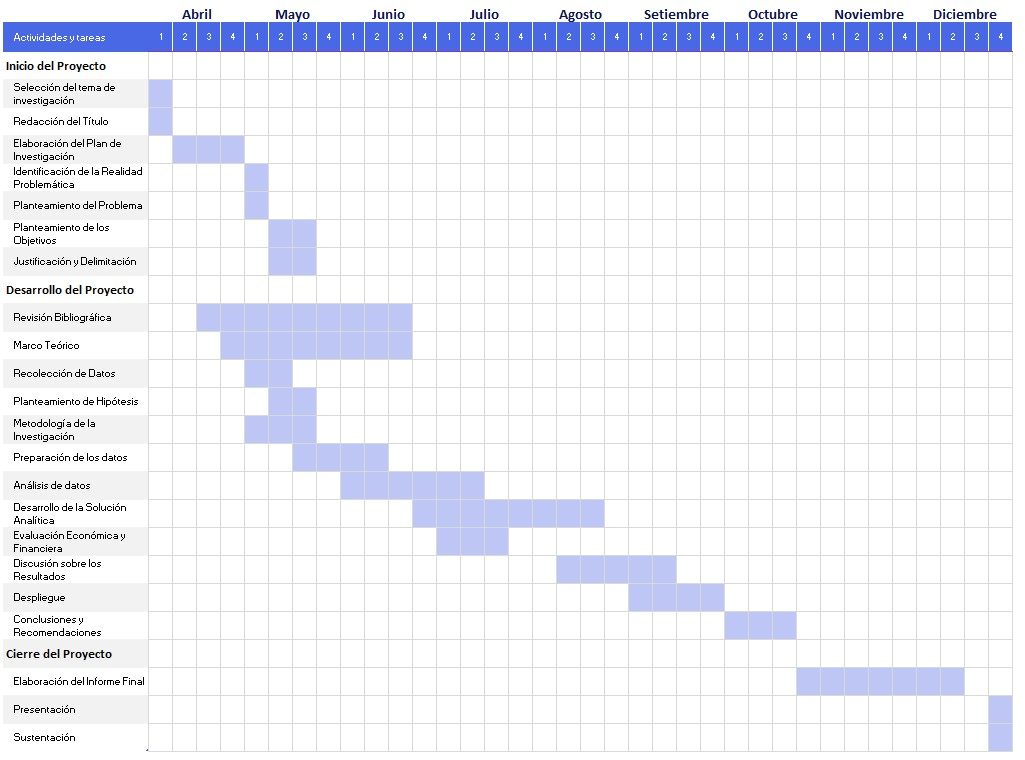
\includegraphics[width=1.35\textwidth]{3/figures/gantt.jpg}
			\caption[Cronograma de actividades]{Cronograma de actividades.\\
				Fuente: Elaboración propia.}
			\label{3:fig1}
		\end{center}
	\end{figure}
	
\end{landscape}

La Tabla 8 ofrece un desglose de los gastos personales del autor de la investigación, incluyendo la adquisición de herramientas como una computadora portátil antes del inicio del proyecto, así como los pagos asociados a servicios generales y al proceso de elaboración y defensa pública de la tesis.

\begin{table}[h!]
	\caption{Presupuesto}
	\label{tab:presupuesto}
	\centering
	\small
	\begin{tabular}{lrrr}
		\toprule
		\textbf{Concepto} & \textbf{Horas empleadas} & \textbf{Gasto (en soles)} & \textbf{Total} \\
		\midrule
		\multicolumn{4}{l}{\textbf{Activos físicos}} \\
		Laptop Lenovo ideapad S340-15IIL Core i7 10va Gen & -- & S/.5,700.00 & S/.5,700.00 \\
		\midrule
		\multicolumn{4}{l}{\textbf{Honorarios por el proceso de elaboración y defensa pública de la tesis}} \\
		Tasa de registro para el tema de investigación & -- & S/.800.00 & S/.800.00 \\
		Apartado del tema de tesis & -- & S/.2,700.00 & S/.2,700.00 \\
		Honorarios de defensa & -- & S/.1,500.00 & S/.1,500.00 \\
		\midrule
		\multicolumn{4}{l}{\textbf{Personal o equipo humano}} \\
		Progreso de tesis & 900 & Incalculable & -- \\
		\midrule
		\multicolumn{4}{l}{\textbf{Gastos operativos}} \\
		Internet + luz (8 meses) & 110 & S/.100.00 & S/.600.00 \\
		\midrule
		\textbf{Total} & -- & -- & S/.11,300.00 \\
		\bottomrule
	\end{tabular}
	%\par	%%Salto de linea
	%\bigskip
	\begin{flushleft}	%%Alinear a la izquierda sin justificar
		\small Fuente: Elaboración propia.
	\end{flushleft}
\end{table}
